% $HeadURL$

\subsection{Glyph: \glyph{Submap terminal}}
\label{sec:submapTerminal}

A \glyph{submap teminal} is a decorator of the \glyph{submap} (\sect{submap}).
It is a named handle, or reference, to both an \glyph{EPN} (\sect{EPNs}) or \glyph{compartment} (\sect{compartment}) of the map, and a \glyph{tag} (\sect{tag}) of the map the \glyph{submap} glyph refers to.
Together with the \glyph{tag}, it allows linking glyphs of a map to their counterpart lying in a submap.

\begin{glyphDescription}

\glyphSboTerm Not applicable.

\add{
\glyphIncoming
One \glyph{equivalence arc} (\sect{equivalenceArc}).
}

\add{
\glyphOutgoing
None.
}

\glyphContainer A \glyph{submap terminal} is represented by a rectangular shape fused to an empty arrowhead, as shown in \fig{submapTerminal}.
The flat edge opposite to the arrowhead should be aligned to the edge of the \glyph{submap} glyph, and the incoming \glyph{equivalence arc} (\sect{equivalenceArc}) should be linked to its middle.

\glyphLabel A \glyph{submap terminal} is identified by a label that is \corr{an unbordered box containing}{} a string of characters \corr{.
The characters}{that} may be distributed on several lines to improve readability.
The centre of the label must be placed on the centre of the \corr{shape}{container}.
The label may extend outside of the \corr{shape}{container}.

\glyphAux
\corr{A \glyph{submap terminal} does not carry any auxiliary items.}{None.}

\end{glyphDescription}

% \begin{figure}[htb]
% \centering
% 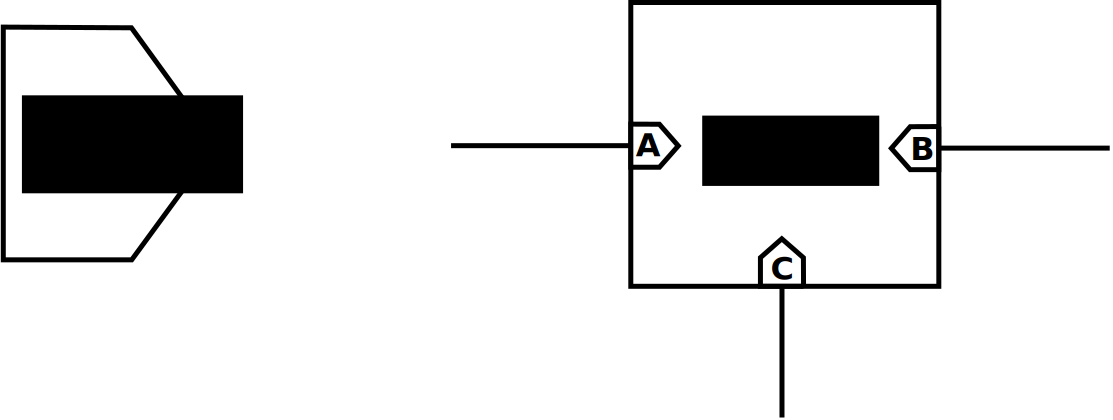
\includegraphics[scale = 0.3]{images/submapterminal}
% \caption{The \PD glyph for \glyph{tag}. This shows the
%   basic glyph and its correct usage within a \glyph{submap} glyph.     }
% \label{fig:tag}
% \end{figure}

\begin{figure}[H]
  \centering
  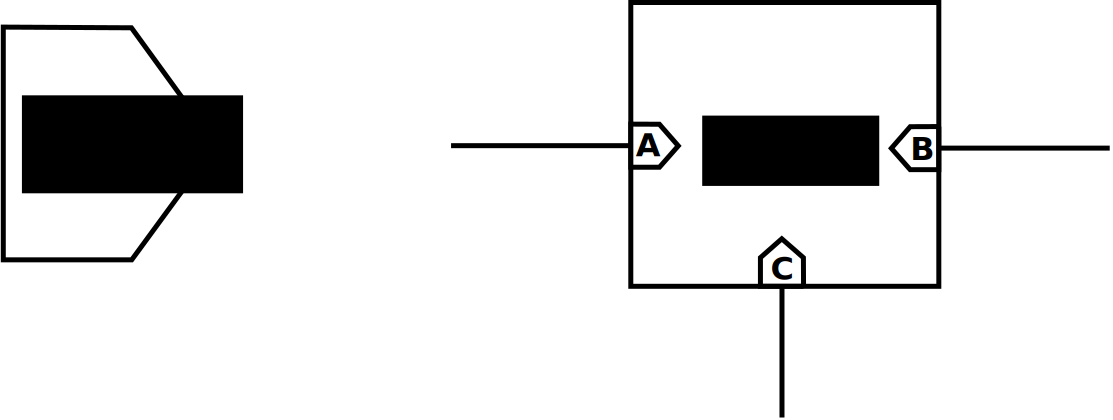
\includegraphics{images/submapterminal}
  \caption{The \PD glyph for \glyph{submap terminal}.}
  \label{fig:submapTerminal}
\end{figure}

% The following is for [X]Emacs users.   Please leave in place.
% Local Variables:
% TeX-master: "../sbgn_PD-level1"
% End:

